\subsection{Explicación de los gráficos}

En los experimentos hechos se realizaron distintos tipos de gráficos

\begin{itemize}
	\item Un gráfico que contiene, en un eje, el promedio de los tiempos totales
	a cada gateway (puntos y lineas rojas), junto con barras verticales rojas
	para indicar la desviación estandar que tuvo esa muestra. A su vez, en el
	mismo grafico, en otro eje, los valores normalizados $Z_{i}$ (ver
	\ref{eq:z}) de cada enlace segun fueron calculados en la metodología y una
	barra horizontal situada en el valor de la tabla $t$ para ese tamaño de
	muestra.  Por encima de este umbral son clasificados los enlaces como
	intercontinentales por el método presentado en este trabajo.  Para
	facilitar la lectura se coloreó con naranja los enlaces que sean
	intercontinentales segun el método propuesto.

	\item Una tabla con las ciudades y paises de donde se localizan las IPS,
	una por cada servicios de geolocalización de IPS para así poder comparar
	los errores cometidos por estos servicios segun el criterio de
	determinación propuesto en este trabajo de los dos tipos de enlaces.

	\item Un mapa con las coordenas por cada servicios de geolocalización de
	IPS ($plotip$ y $geoiptool$) para poder visualizar y contrastar estos
	enlaces desde otra perspectiva que no sean los tiempos de enlace y que
	se complemente con la tabla antes mencionada.
\end{itemize}



\subsection{Universidad de La Habana}

En este experimento analizaremos como se comportan los paquetes enviados hasta la web de la Universidad de La Habana\footnote{http://www.uh.cu/}. Al momento de realizarse el experimento, su IP es 200.55.139.216.

 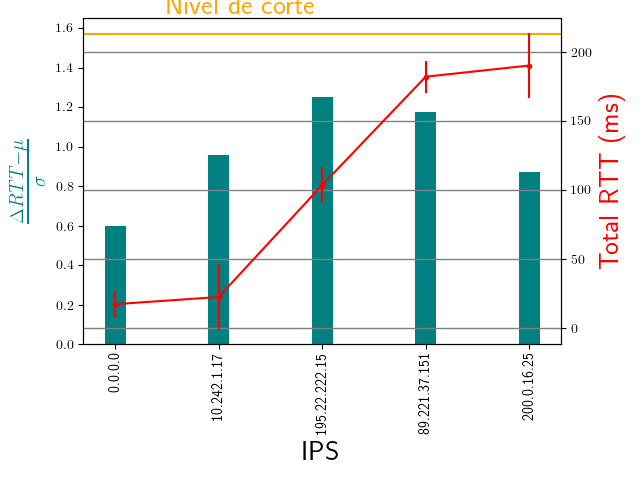
\includegraphics[scale=0.8]{imagenes/rtts_habana.png}

El largo de la ruta es de 5 y en el 100\% de los casos no responde Time exceeded. Adem\'as, podemos observar que ningun cable es considerado transatlantico, utilizando el algoritmo expuesto anteriormente, si bien se puede ver una diferencia considerable de RTT en la IP 195.22.222.15 y 89.221.37.151.  \\

Haremos un mejor an\'alisis utilizando geolocalizaci\'on para intentar entender el camino del paquete. Tanto geoiptool como plotip nos dan dos caminos bastante distintos como muestran las tablas a continuaci\'on
 
\begin{table}
\centering
\begin{tabular}{|c|c|}
10.242.1.17 & No puede procesar \\
195.22.222.15 & Italia  \\
89.221.37.151 & Italia \\
200.0.16.25 & Cuba \\
\end{tabular}
\caption{Utilizando geoiptool}
\end{table}

\begin{table}
\centering
\begin{tabular}{|c|c|c|}
10.242.1.17 & Aachen & Alemania \\
195.22.222.15 & Chicago & Estados Unidos  \\
89.221.37.151 &  & Grecia \\
200.0.16.25 & La Habana & Cuba \\
\end{tabular}
\caption{Utilizando plotip}
\end{table}

Primero vemos que en plotip tiene poco sentido el camino de ir de Alemania a Estados Unidos a Grecia para luego volver a Cuba, adem\'as de que no se condice con los RTTs medidos. Al no poder ser procesada la IP 10.242.1.17 por geoiptool nos hace pensar que el caso de Alemania puede estar mal. Con esto en mente, lo mas factible viendo los resultados de plotip es el camino Buenos Aires - Estados Unidos - Cuba. Descartamos Grecia porque creemos que no tiene sentido hacer ese trayecto por la localizaci\'on tan cercana de Cuba a Estados Unidos.\\

En geoiptool, nos da un camino que puede ser valido ya que es ir a Italia para luego ir a Cuba. Si bien la distancia de Buenos Aires a Estados Unidos es tan grande como la que separa a algunos continentes, resulta raro que no haya detectado ningun camino intercontinental nuestro algoritmo. Esto nos hace ver como mas posible entre ambos caminos el primero. Igualmente es posible que el nivel de corte calculado con el metodo de Cimbala sea muy grande en este caso.\\

Presentamos los graficos generados utilizando la localizaci\'on provista por ambas herramientas para poder comparar visualmente los recorridos.

\begin{figure}
	\centering
 	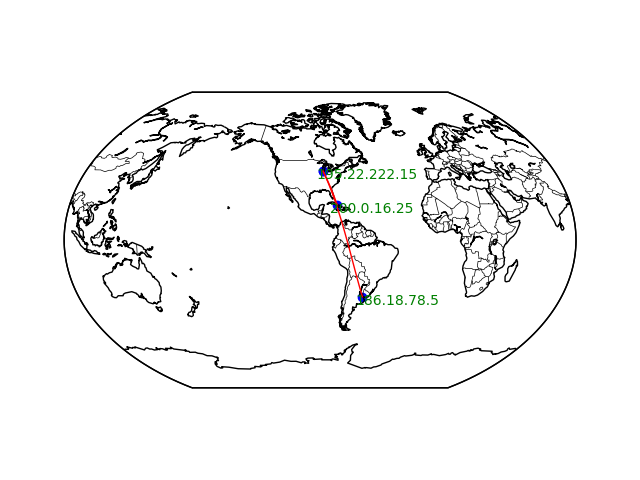
\includegraphics[scale=0.8]{imagenes/mapa_cuba_2.png}
 	\caption{Mapa generado usando plotip para la Universidad de La Habana}
\end{figure} 

\begin{figure}
	\centering
 	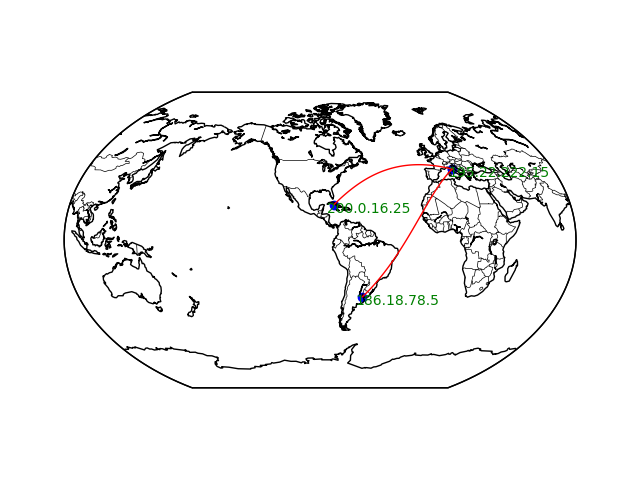
\includegraphics[scale=0.8]{imagenes/mapa_cuba_1.png}
 	\caption{Mapa generado usando geoiptool para la Universidad de La Habana}
\end{figure} 

\subsection{Universidad Estatal de Tomsk - Rusia}

\subsection{Round Trip Times}

\begin{figure}[ht]
	\begin{center}
		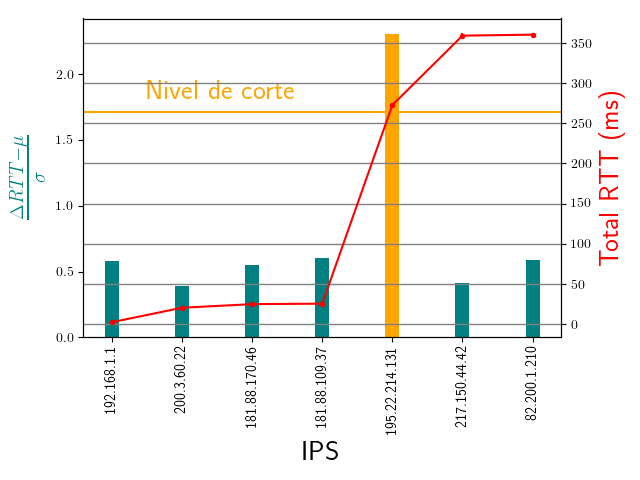
\includegraphics[width=0.8\columnwidth]{imagenes/rtts_tsu.png}
		\caption{Grafico de RTTS totales y de enlaces para la Universidad Estatal de Tomsk}
	\end{center}
\end{figure}

\subsubsection{Mapas}

\begin{tabular}{|c|c|c|c|}
	\hline
	TTL & IP & Ciudad & Pais \\
	\hline
	2 & 200.3.60.22 & Entre Rios & Argentina \\
	\hline
	4 & 181.88.170.46 & & Indonesia \\
	\hline
	5 & 181.88.109.37 & & Indonesia \\
	\hline
	7 & 195.22.214.131 & Bruselas & Bélgica \\
	\hline
	9 & 217.150.44.42 & Khabarovsk & Rusia \\
	\hline
	11 & 82.200.1.210 & Tomsk & Rusia \\
	\hline
\end{tabular}

\begin{tabular}{|c|c|c|c|}
	\hline
	TTL & IP & Ciudad & Pais \\
	\hline
	2 & 200.3.60.22 & Entre Rios & Argentina \\
	\hline
	4 & 181.88.170.46 & Entre Rios & Argentina \\
	\hline
	5 & 181.88.109.37 & Entre Rios & Argentina \\
	\hline
	7 & 195.22.214.131 &  & Italia \\
	\hline
	9 & 217.150.44.42 &  & Rusia \\
	\hline
	11 & 82.200.1.210 & Tomsk & Rusia \\
	\hline
\end{tabular}


\begin{figure}{ht}
	\centering
	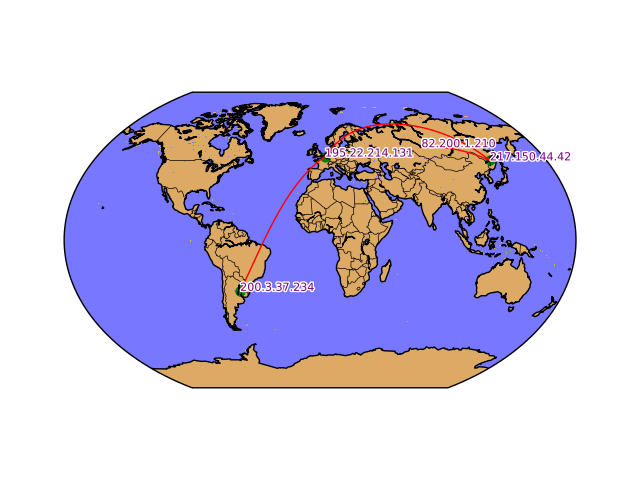
\includegraphics[scale=0.8]{imagenes/mapa_tsu_plotip.png}
	\caption{Mapa generado usando plotip para la Universidad Estatal de Tomsk}
\end{figure} 

\begin{figure}[ht]
	\centering
	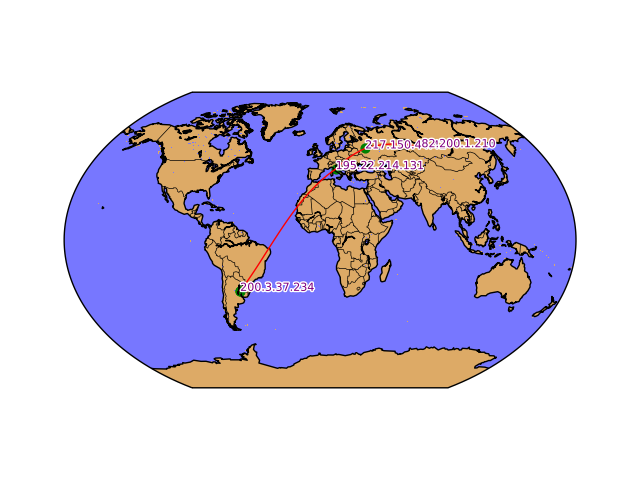
\includegraphics[scale=0.8]{imagenes/mapa_tsu_geoip.png}
	\caption{Mapa generado usando geoiptool para la Universidad Estatal de Tomsk}
\end{figure} 
